\documentclass{article}
\usepackage[utf8]{inputenc}
\usepackage{polski}
\usepackage[polish]{babel}
\usepackage{bbm}
\usepackage{amsmath}
\usepackage{amsthm}
\usepackage{graphicx}
\usepackage{epstopdf}
\usepackage[export]{adjustbox}
\usepackage{float}

\newtheorem{defi}{Definicja}
\newtheorem{twr}{Twierdzenie}
\newtheorem*{dd}{Dowód}

\DeclareMathOperator{\sign}{sign}
\DeclareMathOperator{\arctg}{arctg}

\newcommand{\twopartdef}[4]
{
	\left\{
		\begin{array}{ll}
			#1 & \mbox{jeśli } #2 \\
			#3 & \mbox{jeśli } #4
		\end{array}
	\right.
}


\author{Jarosław Dzikowski 273233}
\date{Wrocław, \today}
\title{\textbf{Bazy danych} \\ Rowery miejskie - model konceptualny} 
\begin{document}
\maketitle

\section{Diagram E-R}
\pagenumbering{gobble}% Remove page numbers (and reset to 1)
%\clearpage
\begin{figure}[p]
\centerline{	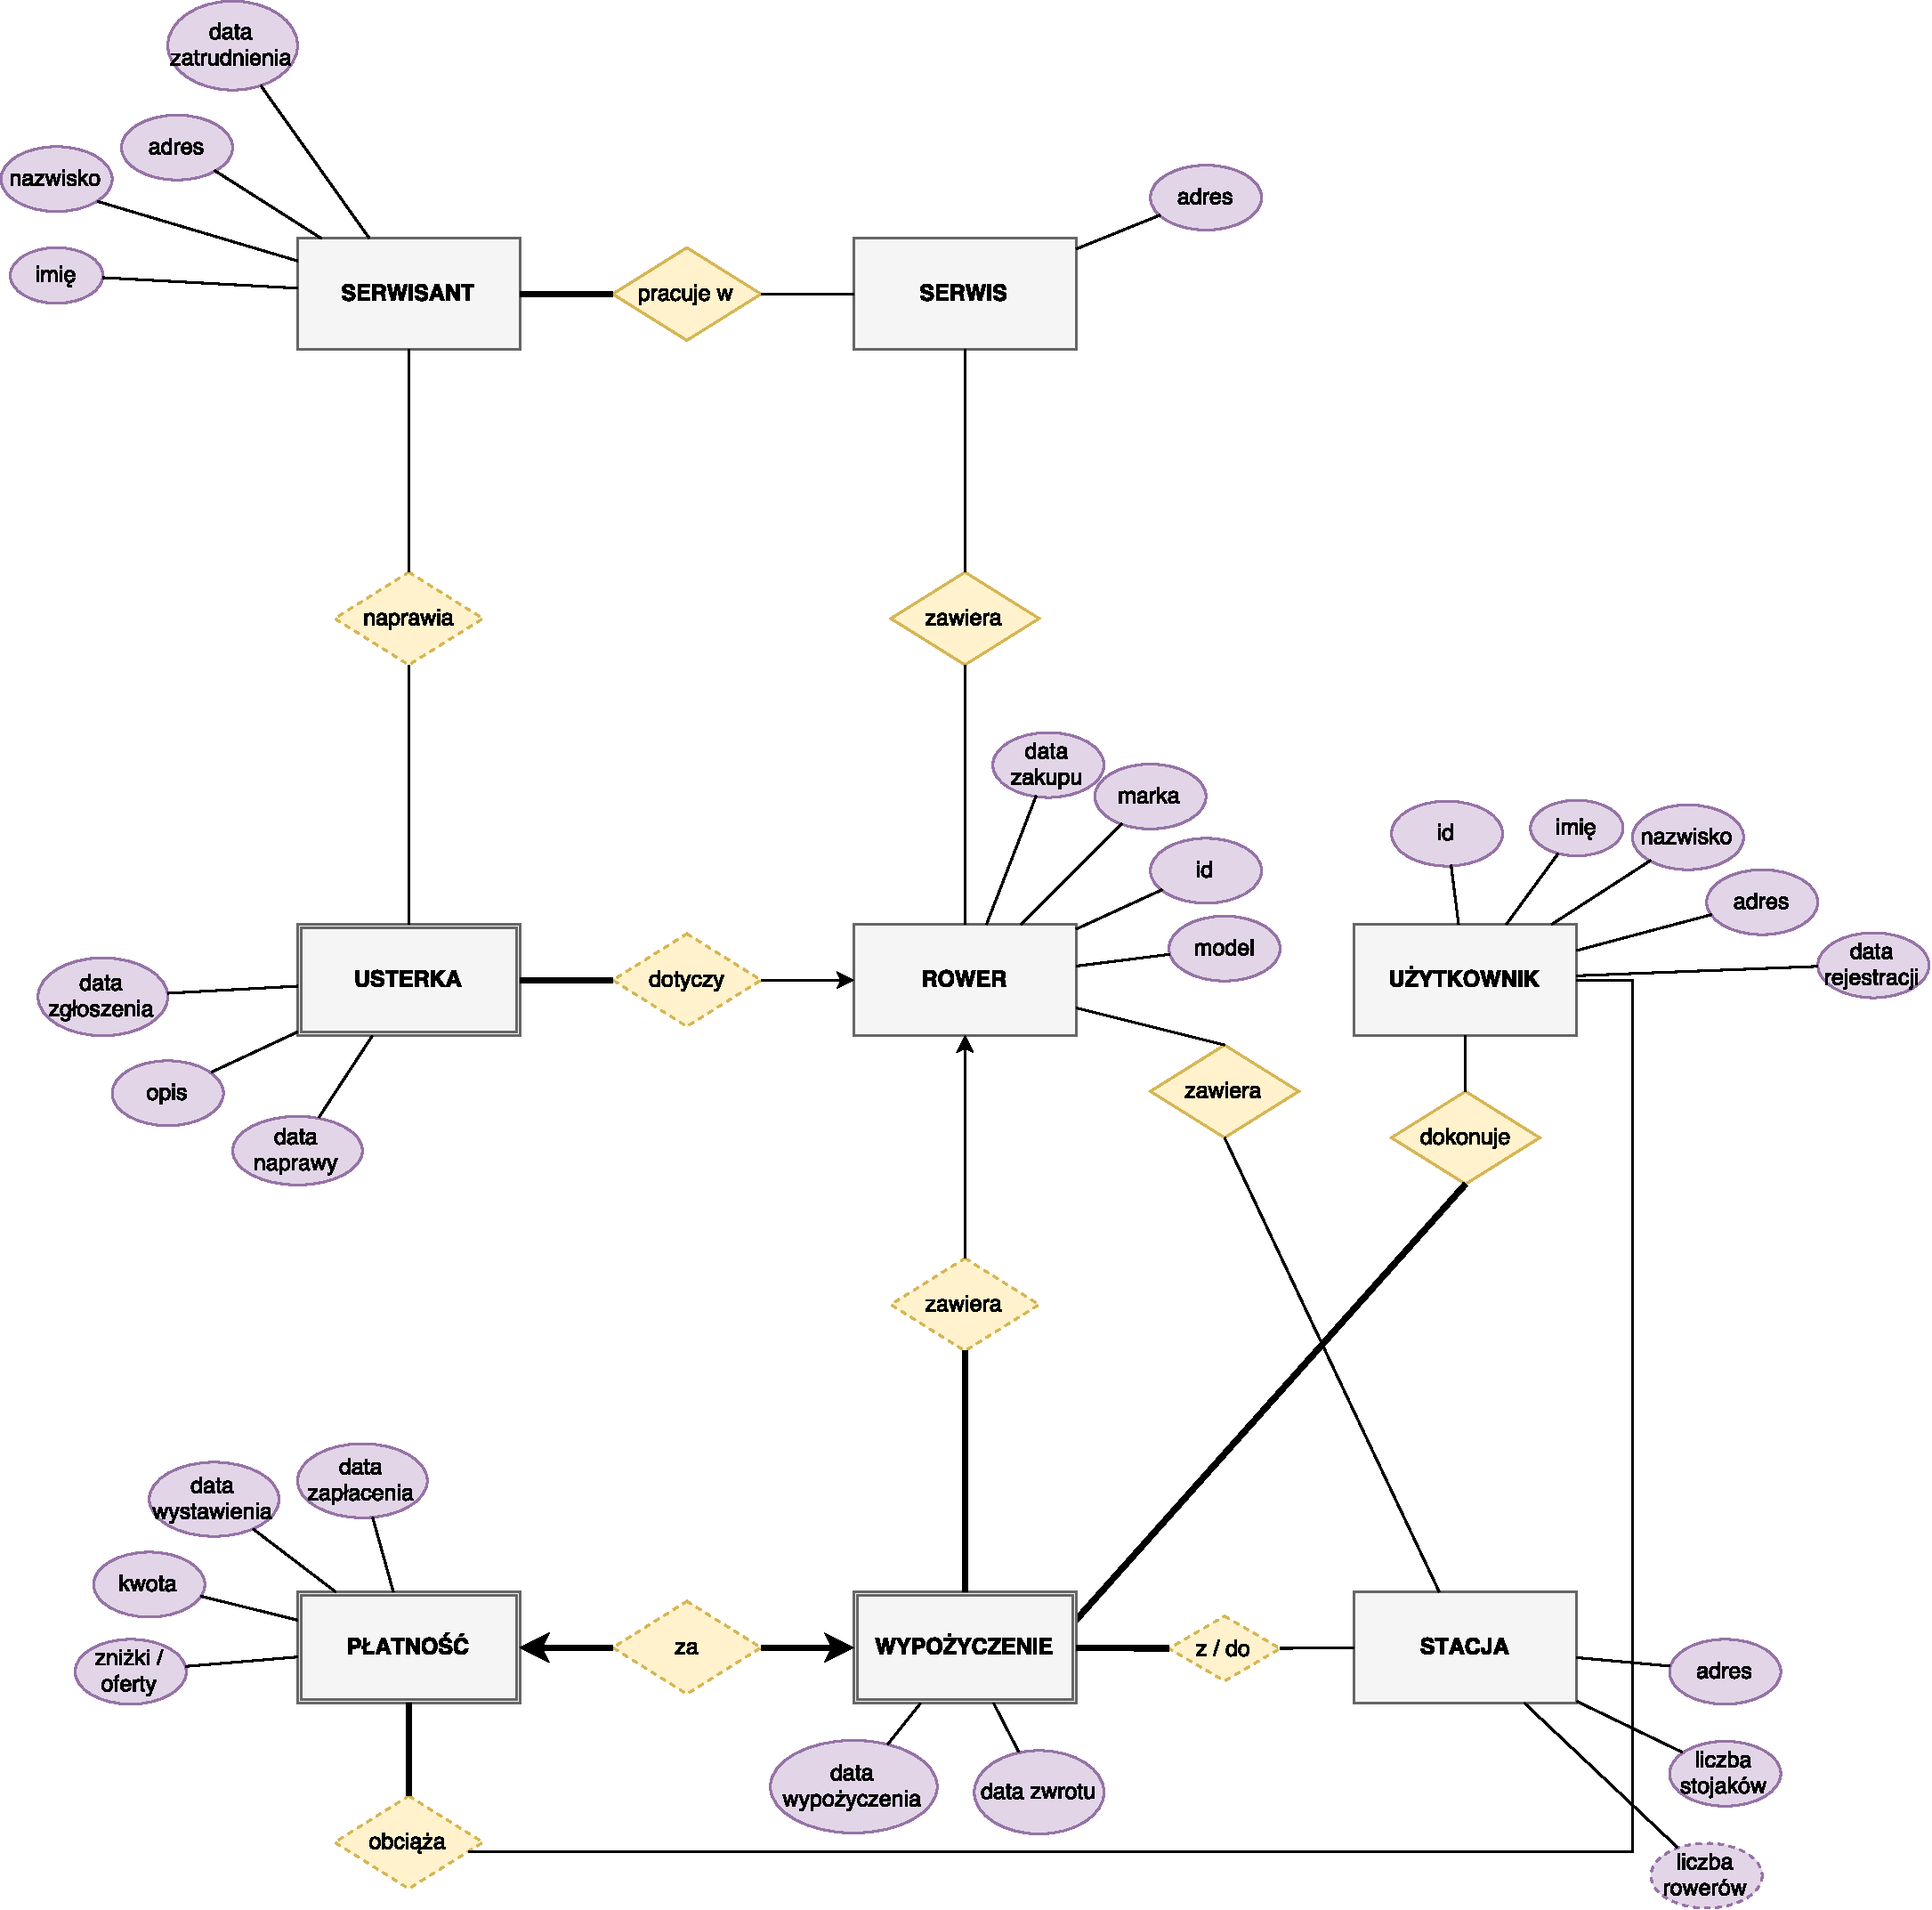
\includegraphics[width=\paperwidth, height=\paperheight, keepaspectratio]{diagram.pdf}}
\end{figure}
\section{Wprowadzenie}


\end{document}
